\chapter{Nástroj Node-RED}
\label{ch:nastroj-node-red}

Node-RED je nástroj tvůrci popsaný jako \uv{Flow-based programming for the Internet of Things}, tedy nástroj založený na
programování na datovém toku určený pro IoT. Uživateli-programátorovi nabízí jednotlivé funkční bloky (či \emph{uzly} dle kontextu),
jejichž vstupy a výstupy lze vzájemně propojovat a vytvářet tak síť jakožto celek s~požadovanými funkcemi.
V~roce 2013 jej představila společnost IBM v~rámci projektu JS Foundation pod licencí Apache 2.0. Nástroj vyžaduje
běhové prostředí Node.js, tedy je naimplementován v~programovacím jazyke Javascript, od čehož se odvíjí možnosti
rozšiřování.

\begin{figure}
    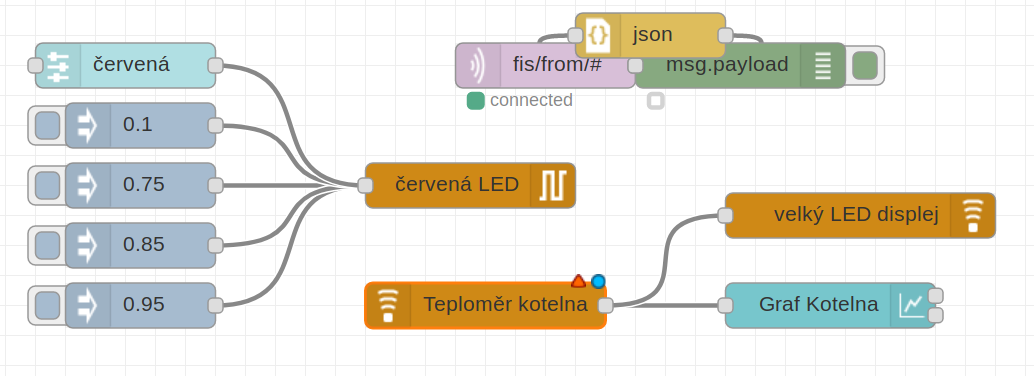
\includegraphics[width=\textwidth]{figures/node-red-example.png}
    \label{fig:node-red-example}
    \caption{Ukázka z~Node-RED -- vstupy a výstupy jednotlivých uzlů spojené pro vzájemnou komunikaci.}
\end{figure}

\subsection{Programování datového toku}
Programovací paradigma založené na editaci datového toku bylo popsáno v~již v dubnu roku 1974 vědcem Dennisem. Jeho
principem je programování pomocí vytváření datových spojů mezi funkčními bloky.
Ve své knize \uv{First Version of a Data Flow Procedure Language}~\cite{FirstVersionOfDataflow} popisuje sémantický
význam funkčních bloků propojených pomocí propojů, které zajištují vzájemnou komunikaci. \todo{Dataflow/flow based
programming}
\blind{2}

\section{Základní principy Node-RED}\label{sec:zakladni-principy-node-red}

\todo{Pouziti, opensource}
Vnitřní architektura nástroje Node-RED je rozdělena na dva samostatné funkční části.
V~pohledu samotného běhu je důležitější částí jádro provádějící veškeré datové operace nad samotným nadefinovaným
modelem, zodpovědné za spouštění jednotlivých uživatelských uzly, jejich synchronizaci a vzájemnou distribuci dat.
Druhou částí je samotný vizuální editor, který je ve výchozím nastavení dostupný pomocí protokolu HTTP. Pomocí něj je
možné uživatelsky nastavovat jednotlivé uzly a vytvářet mezi nimi datové spoje.

Toto rozdělení nabízí možnost běhu sítě mimo samotný editor, a to především kvůli bezpečnostním a
výkonnostním důvodům -- každé \uv{flow} (množina entit funkčních uzlů a jejich propojení, dále jen
\emph{sít}\footnote{Pro \uv{flow} by se dal uvažovat taktéž překlad \uv{tok},
příp. přímo \uv{datový tok}, což ale příliš nekoresponduje s~praktickou stránkou věci -- \uv{síť} je reprezentativnější
pojmenování pro strukturu vytvářenou editorem, i například vzhledem k~pojmenování Petriho sítí.}) je schopen
Node-RED serializovat do formátu JSON, tedy i ukládat či načítat do, resp. ze souborů, díky čemuž lze jednotlivé
sítě i snadno sdílet.

Mechanika samotných zpráv a jejich doručování je založena na několika základních premisách:
\begin{enumerate}
    \item Zprávy jsou obecně \emph{Javascript} hodnoty, v~naprosté většině případů datového typu \ic{Object},
    tedy množiny dvojic \emph{klíč-hodnota}.
    \item Každý z~funkčních uzlů může vlastnit $0-N$ vstupních portů, stejně tak $0-M$ výstupních portů.
    \item Jednotlivé výstupy a vstupy lze propojovat, a to i vícenásobně, tedy více výstupů lze připojit na jeden vstup,
    stejně tak z~jednoho výstupu lze použít spojení do více vstupů.
    \item Zodpovědností uzlů je provedení deterministicky definované funkce na základě přijaté zprávy nebo
    jiného externího vstupu.
    \item Zodpovědností sítě je distribuce zpráv mezi uzly a jejich asynchronní spouštění.
\end{enumerate}

Node-RED bez dalších rozšíření nabízí základní sadu uzlů, mezi ty nejobecněji použitelné patří:

\begin{itemize}
    \item\emph{function} -- Blok vykonávající nakonfigurovaný uživatelský kód v~programovacím jazyce Javascript pro
    každou příchozí zprávu.
    \item\emph{inject} -- Interaktivní blok umožnující uživateli editoru zaslat konkrétní zprávu na výstup tohoto bloku
    přímo z~editoru (tedy internetového prohlížeče) -- vhodné především pro testování či manuální zasílání zpráv.
    \item\emph{debug} -- Blok poskytující logovací službu, dle jeho konfigurace jsou přijaté zprávy logovány do systémové konzole či do
    bočního panelu v~editoru -- blok vhodný pro testování a monitorování stavu sítě.
    \item\emph{switch} -- Jeden z~bloků starajících se o~směrování zpráv v~síti -- na základně definovaných pravidel
    (shoda či porovnání hodnot, regulární výrazy) rozhodne, který z~výstupů bude použit pro další směřování zprávy.
    \item\emph{delay} -- Blok umožňující časové operace nad tokem zpráv zkrz tento blok - dle konfigurace zprávy buď
    pouze zpožďuje o~konstantní hodnotu, nebo i omezuje průtok (šířku pásma) za časovou jednotku.
\end{itemize}

Pro bloky využívající externí služby nabízí Node-RED institut konfiguračních bloků.
S pomocí nich je možné sdílet a znovupoužívat statickou konfiguraci v dalších blocích -- tedy např. údaje pro
připojení k MQTT brokeru není nutné zadávat do každého bloku zvlášť, ale jsou sdílené pro jeden konfigurační blok,
který je následně přiřazen ke každému bloku vyžadující MQTT broker.

\begin{figure}%
    \centering
    \subfloat[konfigurace výstupního MQTT bloku -- modře zvýrazněn vybraný MQTT broker]%
    {{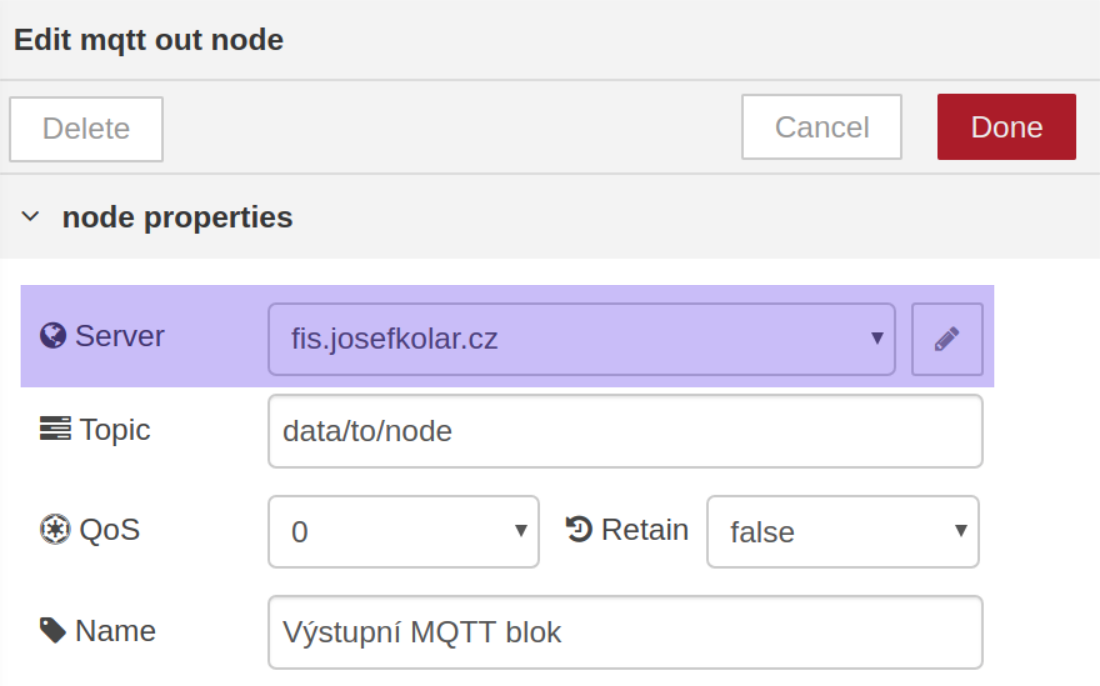
\includegraphics[valign=t,width=.45\textwidth]{figures/node-red-mqtt-out-conf.png}}}%
    \qquad
    \subfloat[konfigurace připojení k MQTT brokeru -- konfigurační blok]%
    {{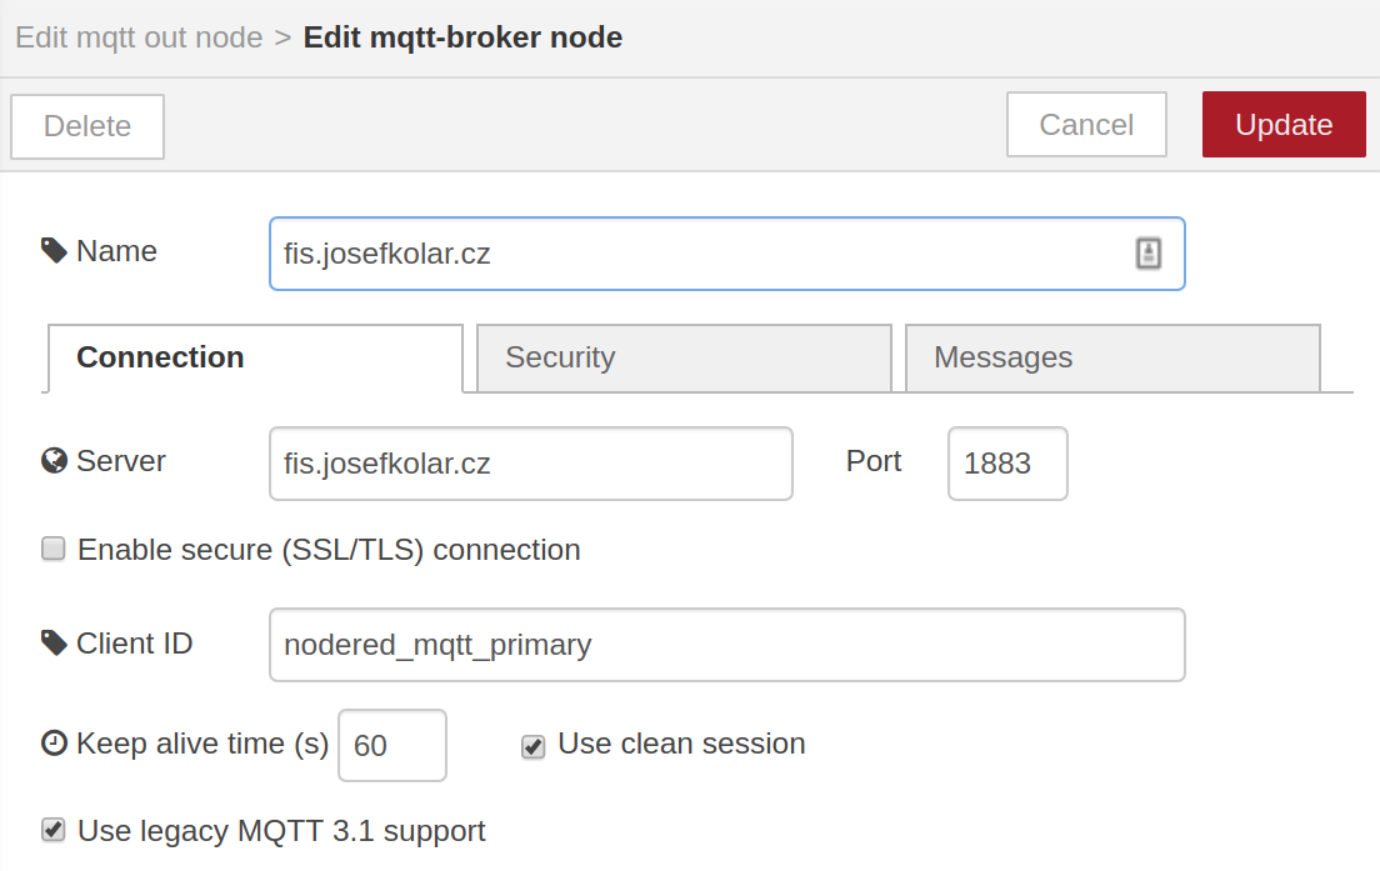
\includegraphics[valign=t,width=.45\textwidth]{figures/node-red-mqtt-broker-conf.png} }}%
    %
    \caption{%
    Konfigurace výstupního MQTT bloku zahrnuje nastavení celého bloku (výstupní kanál, QoS, příznak \uv{retain}
    či pojmenování samotného bloku) a nastavení samotného MQTT připojení (cílový server, identifikace klienta či
    autentizační údaje)
    }%
    \label{fig:node-red-mqtt-out-conf}
    %
\end{figure}


\section{Rozšíření pomocí vlastních modulů}\label{sec:rozšíření-pomocí-vlastních-modulů}

Díky povaze nástroje Node-RED


\todo{Rozšíření pomocí vlastních modulů}


\missingfigure{Node-RED spojeni}
